\chapter{緒論}
\label{chapter:intro}
\section{研究背景與動機}
\label{sec:background}
    \subsection{子章節一}
        字章節一段落一,字章節一段落一,字章節一段落一,字章節一段落一,
        字章節一段落一,字章節一段落一,字章節一段落一,字章節一段落一,
        字章節一段落一,字章節一段落一,字章節一段落一,字章節一段落一,
        字章節一段落一,字章節一段落一,字章節一段落一,字章節一段落一,
        字章節一段落一,字章節一段落一,字章節一段落一。

        字章節一段落二,字章節一段落二,字章節一段落二,字章節一段落二,
        字章節一段落二,字章節一段落二,字章節一段落二,字章節一段落二,
        字章節一段落二,字章節一段落二,字章節一段落二,字章節一段落二,
        字章節一段落二,字章節一段落二,字章節一段落二,字章節一段落二,
        字章節一段落二,字章節一段落二,字章節一段落二,字章節一段落二,
        字章節一段落二,字章節一段落二,字章節一段落二,字章節一段落二,
        字章節一段落二。

        例如現有的系統有\cite{GoogleComputeEngine}、\cite{AmazonEC2}等等,
        另外\cite{GoogleApps}是以○○○技術來達成。

        ○○系統結構如示意圖\ref{fig:this_system}
        \begin{figure}[htbp]
            \centerline{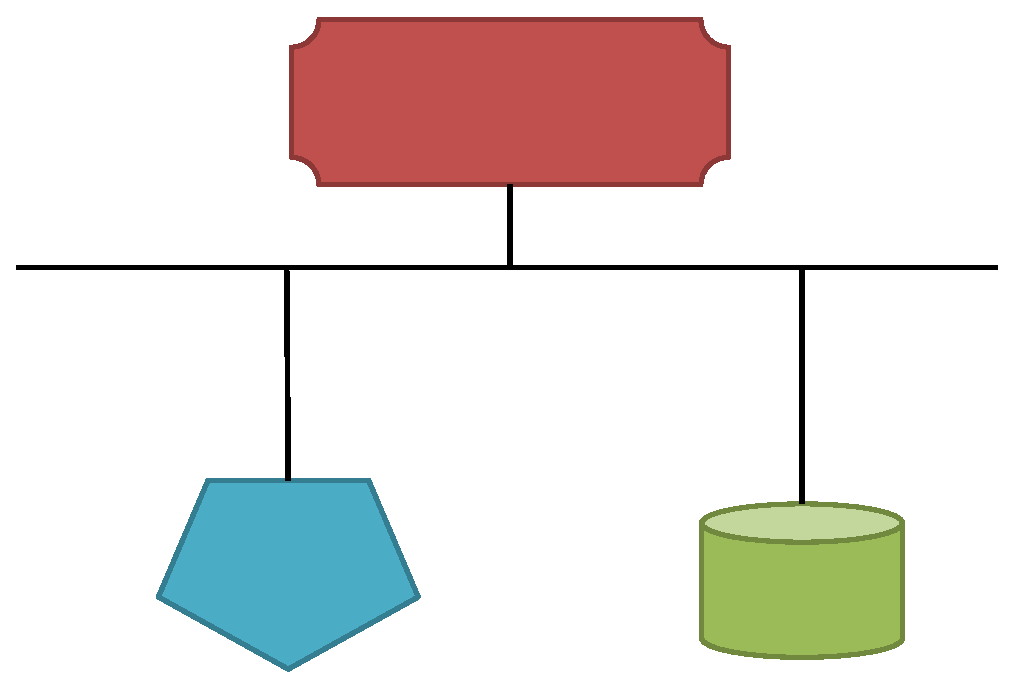
\includegraphics[height=5cm]{graphs/introduction/this_system.eps}}
            \caption{○○示意圖}
            \label{fig:this_system}
        \end{figure}

    \subsection{子章節二}
        字章節二,字章節二,字章節二,字章節二,字章節二,
        字章節二,字章節二,字章節二,字章節二,字章節二,
        字章節二,字章節二,字章節二,字章節二,字章節二,
        字章節二,字章節二,字章節二,字章節二,字章節二,
        字章節二,字章節二,字章節二,字章節二,字章節二,
        字章節二,字章節二,字章節二,字章節二,
        ○○○如圖~\ref{fig:types_comparison}所示。
        \begin{figure}[!t]
            \begin{center}
                \begin{tabular}{ccccccccccccc}
                    \subfigure[類型A]{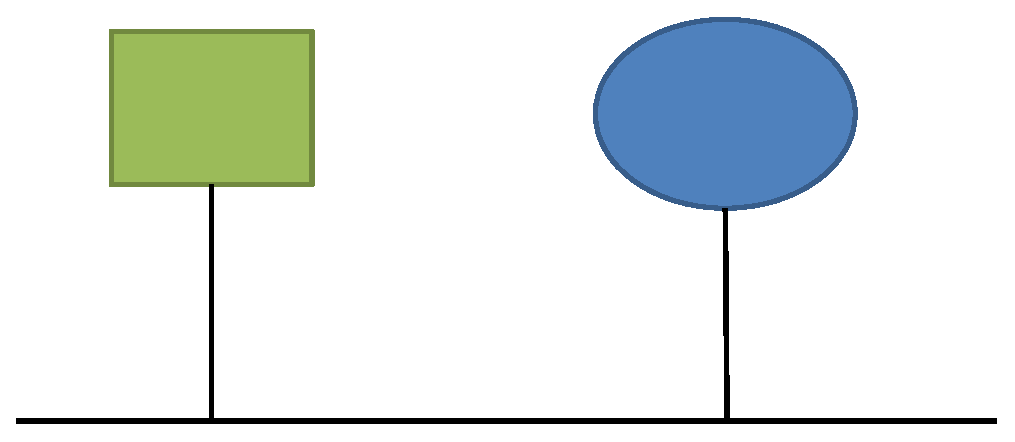
\includegraphics[height=2.4cm]{graphs/introduction/typeA.eps}\label{fig:typeA} } \par &
                    \subfigure[類型B]{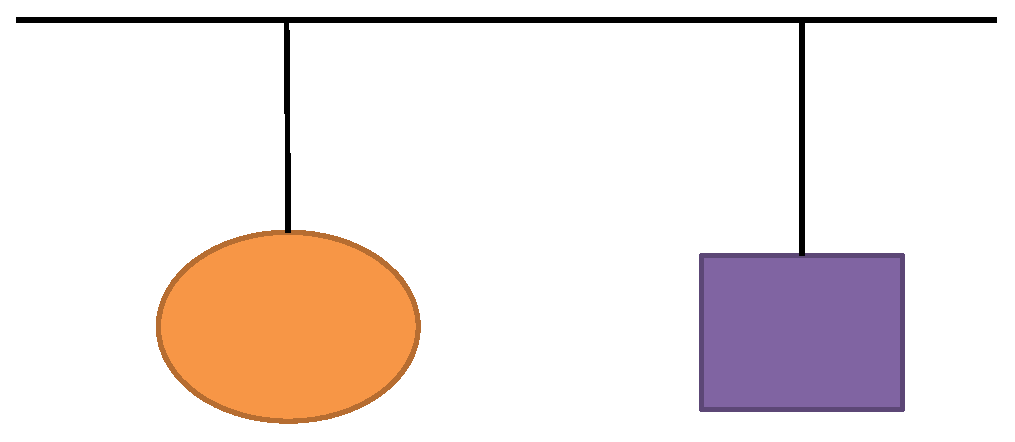
\includegraphics[height=2.4cm]{graphs/introduction/typeB.eps}\label{fig:typeA} } \par \\
                \end{tabular}
                \caption{○○○比較}
                \label{fig:types_comparison}
            \end{center}
        \end{figure}

\section{○○○問題與處理機制}
    問題與機制,問題與機制,問題與機制,問題與機制,
    問題與機制,問題與機制,問題與機制,問題與機制,
    問題與機制,問題與機制,問題與機制,問題與機制,
    問題與機制,問題與機制,問題與機制,問題與機制,
    問題與機制。

    %要被單行註解的文字。

\begin{comment}
    要被區塊註解的文字,要被區塊註解的文字,要被區塊註解的文字,
    要被區塊註解的文字,要被區塊註解的文字,要被區塊註解的文字,
    要被區塊註解的文字,要被區塊註解的文字,要被區塊註解的文字,
    要被區塊註解的文字,要被區塊註解的文字,要被區塊註解的文字,
    要被區塊註解的文字,要被區塊註解的文字,要被區塊註解的文字,
    要被區塊註解的文字,要被區塊註解的文字。
\end{comment}

\section{研究動機與目的}
    動機與目的,動機與目的,動機與目的,動機與目的,
    動機與目的,動機與目的,動機與目的,動機與目的,
    動機與目的,動機與目的,動機與目的,動機與目的,
    動機與目的,動機與目的,動機與目的,動機與目的,
    動機與目的,動機與目的,動機與目的,
    細節如表\ref{tab:mytitle1}。
    \begin{table}[!t]
        \centering
        \caption{表格標題1}
        \label{tab:mytitle1}
        % Table generated by Excel2LaTeX from sheet 'table_01'
\begin{tabular}{rr}
\toprule
Title & Values \\
\midrule
A     & 1612 \\
B     & 256 \\
C     & 30 \\
D     & 7 \\
E     & 3 \\
\bottomrule
\end{tabular}%

    \end{table}

    \begin{enumerate}
        \item
        列舉一。
        %
        \item
        列舉二。
        %
        \item
        列舉三。
        %
    \end{enumerate}

\section {研究方法與論文架構}
    研究方法與論文架構,研究方法與論文架構,研究方法與論文架構,
    研究方法與論文架構,研究方法與論文架構,研究方法與論文架構,
    研究方法與論文架構,研究方法與論文架構,研究方法與論文架構,
    研究方法與論文架構。

    \begin{itemize}
        \item
        項目一。
        %
        \item
        項目二。
        %
        \item
        項目三。
        %
        \item
        項目四。
    \end{itemize}

    流程圖如\ref{fig:ResearchFlowChart}。
    \begin{figure}[htbp]
        \centering
        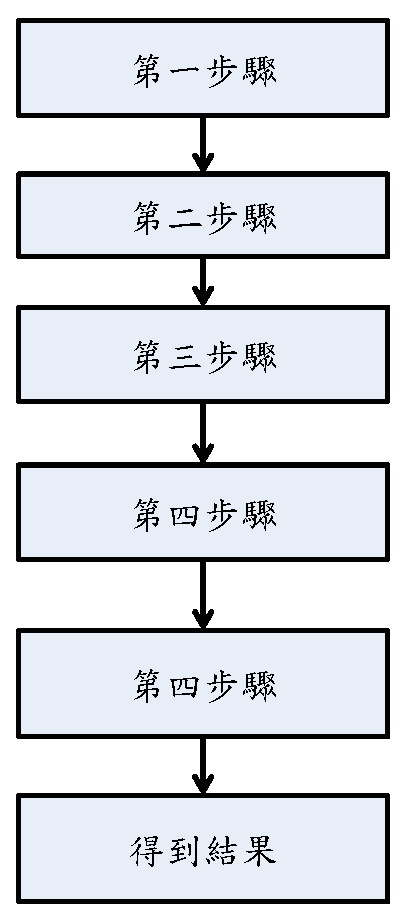
\includegraphics[height=8cm]{graphs/introduction/ResearchFlowChart.eps}
        \caption{研究進行流程圖}
        \label{fig:ResearchFlowChart}
    \end{figure}

